\documentclass[conference]{IEEEtran}
\IEEEoverridecommandlockouts

\usepackage{amsmath,amssymb,amsfonts}
\usepackage{graphicx}
\usepackage{textcomp}
\usepackage{xcolor}
\usepackage{booktabs}
\usepackage{array}
\usepackage[hyphens]{url}
\usepackage[numbers,sort&compress]{natbib}
\usepackage{hyperref}

\hypersetup{
  colorlinks=true,
  citecolor=blue!60!black,
  linkcolor=blue!50!black,
  urlcolor=blue!50!black
}

% Measured results from the reported run (src/train.py --subset 0.09 --epochs 2).
\newcommand{\TBD}[1]{\textcolor{red}{\textbf{[#1]}}}
\newcommand{\ValAcc}{63.86\%}
\newcommand{\ValP}{66.25\%}
\newcommand{\ValR}{63.86\%}
\newcommand{\ValF}{63.67\%}
\newcommand{\TestAcc}{63.15\%}
\newcommand{\TestP}{64.73\%}
\newcommand{\TestR}{63.15\%}
\newcommand{\TestF}{62.85\%}
\newcommand{\TrainWall}{1~h 42~min}
\newcommand{\TrainRate}{11.6 samples/s}
\newcommand{\TrainLoss}{0.850}
\newcommand{\EpOneAcc}{57.35\%}
\newcommand{\EpTwoAcc}{63.86\%}

\begin{document}

\title{Cross-Lingual Textual Entailment for Hindi:\\
Adapting Lexical Matching to XLM-RoBERTa Fine-Tuning}

\author{\IEEEauthorblockN{Mohammed Ufraan}
\IEEEauthorblockA{\textit{Department of Computer Science}\\
Lords Institute of Engineering \& Technology\\
naarfu@gmail.com}
}

\maketitle

\begin{abstract}
Recognizing textual entailment (RTE) asks whether the meaning of a hypothesis can be inferred from a premise. \citet{khader2016textual} addressed this problem for Arabic with stemmed word overlap, synonym expansion, and bigram thresholds, reporting 61\% overall precision and recall on a 100-pair sample of ArbTEDS. We keep their scientific question - entailment outside English, in a morphologically rich language - but change the language, data, algorithm, and training method. Specifically, we fine-tune XLM-RoBERTa-base on the Hindi split of XNLI for three-way natural language inference (entailment, neutral, contradiction). Evaluation uses the standard 5{,}010-pair XNLI-Hindi test set rather than a 100-pair subsample. On Apple Silicon we document a training-stack failure (fused AdamW and SDPA) that collapsed the classifier to chance (33.3\% accuracy, loss pinned at $\ln 3$), and we replace it with eager attention and unfused AdamW. After two epochs over 9\% of the Hindi train split (35{,}343 pairs, $\approx$1\,h~42\,min), the model reaches \TestAcc{} test accuracy and \TestF{} macro-F1.
\end{abstract}

\begin{IEEEkeywords}
textual entailment, natural language inference, Hindi, XLM-RoBERTa, XNLI, transfer learning
\end{IEEEkeywords}

\section{Results summary}
\label{sec:checklist}
All reported numbers are measured. The sanity 5\%/1-epoch numbers and the reported 9\%/2-epoch numbers come from the training and evaluation logs reproduced in Section~\ref{sec:exp}. No mock values remain in this document.

\section{Introduction}
\label{sec:intro}

Textual entailment, also called natural language inference (NLI), is the problem of deciding whether a hypothesis $H$ is true given a text or premise $T$~\citep{dagan2006rte,bowman2015snli}. A system that cannot tell whether one sentence licenses another cannot reliably summarize, answer questions, or filter retrieved passages: those applications all reduce, at some step, to ``does this sentence follow from that one?''

The PASCAL Recognising Textual Entailment challenges~\citep{dagan2006rte} framed the modern English evaluation as a two-way decision (\emph{entails} / \emph{does not entail}). Later English corpora, especially SNLI~\citep{bowman2015snli} and MultiNLI~\citep{williams2018snli}, added a third \emph{neutral} label for cases where $T$ neither supports nor contradicts $H$. Most published neural NLI work still concentrates on English. Work on Arabic, Hindi, and other morphologically rich languages remains thinner, even though those languages are exactly where surface-form matching is least reliable.

\subsection{The paper we adapt}
\citet{khader2016textual} studied RTE for Arabic. Arabic has optional diacritics (so a single undiacritized token can have several readings), flexible word order (VSO, SVO, and others), and a large synonym inventory. Their system is a pipeline of preprocessing (named-entity marks, POS tags from MSTParser and MADA, ISRI stemming), stop-word removal, unigram overlap with synonym credit, and hypothesis-normalized bigram overlap. Each overlap score is compared to a threshold chosen on a development sample. The decision is binary: Entails or NotEntails. On 100 randomly selected pairs from ArbTEDS~\citep{alabbas2013dataset} they report 68\% precision / 64\% recall for Entails, 58\% / 60\% for NotEntails, and 61\% overall precision and recall (their Table~6; 61 of 100 pairs judged correctly in their Table~5).

That design has four structural limits. First, thresholds and bag-of-word overlap do not model long-range context or compositional negation. Second, the authors themselves note, following \citet{alkhawaldeh2015negation}, that treating negation as a stop word can reverse polarity. Third, evaluation is a 100-pair subsample of a 618-pair corpus, so confidence intervals are wide. Fourth, the feature stack (ISRI stemmer, Arabic WordNet-style synonyms, CoNLL trees) does not transfer to Hindi.

\subsection{What we change}
We keep the same research question - can we recognize entailment in a morphologically rich language other than English - and change the implementation along five axes of the original design (Table~\ref{tab:options}). Hindi, like Arabic, has rich morphology and relatively free word order, and it is written in Devanagari rather than Arabic script, so a successful transfer cannot be a copy-paste of stemmers and lexicons. We therefore replace the lexical pipeline with a pretrained multilingual Transformer~\citep{conneau2020xlmr} fine-tuned on XNLI Hindi~\citep{conneau2018xnli}.

\begin{table}[!t]
\centering
\caption{Six ways this work differs from the original system.}
\label{tab:options}
\begin{tabular}{@{}clp{0.58\linewidth}@{}}
\toprule
\# & \textbf{Option} & \textbf{This work} \\
\midrule
1 & Different language & Arabic $\rightarrow$ Hindi \\
2 & Improved results & 61\% P/R $\rightarrow$ \TestAcc{} test acc. \\
3 & Changed algorithm & Overlap rules $\rightarrow$ Transformer \\
4 & Changed methodology & Thresholds $\rightarrow$ gradient fine-tuning \\
5 & Full implementation & Runnable data-processing, training, and evaluation scripts \\
6 & Different dataset & ArbTEDS $\rightarrow$ XNLI Hindi \\
\bottomrule
\end{tabular}
\end{table}

Option~2 must be stated carefully. \citet{khader2016textual} report two-way precision/recall on 100 Arabic pairs. We report three-way accuracy on 5{,}010 Hindi pairs. If our test accuracy is well above 61\%, the original system's score is improved upon, but it is \emph{not} a matched leaderboard. Published XLM-R-base scores on XNLI-Hindi sit in the mid-70\% range~\citep{conneau2020xlmr}; that is the honest target. An 85\%+ claim would require a larger model or extra data and is not assumed here.

\subsection{Contributions}
This report makes four concrete contributions:
\begin{enumerate}
  \item A complete, runnable fine-tuning recipe for XLM-RoBERTa-base on XNLI Hindi (batch 16, length 128, learning rate $2\times 10^{-5}$, 10\% warmup, two epochs over 9\% of the train split).
  \item A documented MPS failure mode: default fused AdamW in Transformers v5 plus SDPA produced a collapsed $\langle s\rangle$ representation, training loss $\approx \ln 3$, and 33.33\% validation accuracy with macro-precision 0.111. The fix is eager attention and unfused AdamW.
  \item A comparison, with caveats, against the Arabic lexical baseline of \citet{khader2016textual}.
  \item An IEEE-format write-up and public scripts so the experiment can be reproduced on Apple Silicon without a CUDA GPU.
\end{enumerate}

Section~\ref{sec:related} reviews RTE, Arabic TE, and multilingual encoders. Section~\ref{sec:hindi} sketches why Hindi is a fair analogue of Arabic for this study. Section~\ref{sec:khader} reconstructs the original lexical method. Section~\ref{sec:data} describes XNLI Hindi. Section~\ref{sec:method} specifies the model and optimizer. Section~\ref{sec:exp} gives the experimental protocol. Section~\ref{sec:results} reports measured results. Section~\ref{sec:disc} discusses limitations and Section~\ref{sec:conc} concludes.

\section{Related Work}
\label{sec:related}

\subsection{English RTE and NLI}
Early RTE systems mixed WordNet, logical inference, n-gram overlap, and syntactic matching~\citep{dagan2006rte}. Overlap-based systems combine unigram overlap with WordNet and give extra weight to POS and named entities - a recipe close to \citet{khader2016textual}. \citet{pakray2011textual} add an SVM over 23 lexical features plus a rule-based syntactic tag, scoring the mid-50s on RTE-4. These systems show that overlap is a surprisingly strong baseline when $T$ and $H$ share many content words, and a weak one when entailment depends on a single negation, a paraphrase, or a world-knowledge fact.

Large annotated corpora changed the method. SNLI~\citep{bowman2015snli} provided hundreds of thousands of English pairs; MultiNLI~\citep{williams2018snli} added genre diversity. Neural classifiers trained on those corpora quickly overtook feature pipelines. BERT~\citep{devlin2019bert} made the standard recipe: concatenate $T$ and $H$, encode with a Transformer~\citep{vaswani2017attention}, and classify the first-token state. RoBERTa~\citep{liu2019roberta} kept the architecture and improved the pretraining recipe (more data, no next-sentence prediction, dynamic masking).

\subsection{Arabic textual entailment}
Arabic TE is small as a literature. \citet{alabbas2011arbte} first laid out why off-the-shelf English RTE tools fail on Arabic (diacritics, flexible order, parser noise) and experimented with tree-edit distance on dependency trees. \citet{alabbas2013jair} extend TED with subtree operations. ArbTEDS~\citep{alabbas2013dataset} collects 618 news headline--article pairs, triple-annotated, covering sport, politics, business, and general news. \citet{alkhawaldeh2015negation} show that dropping Arabic negation as a stop word flips Entails/NotEntails. \citet{khader2016textual} sit in this line: they keep the ArbTEDS setting and a lexical/semantic pipeline rather than TED, and they evaluate with RTE-2 style precision and recall.

\subsection{Cross-lingual NLI and XLM-R}
XNLI~\citep{conneau2018xnli} translates MultiNLI development and test data into 14 other languages (15 including English), among them Hindi, and provides a training corpus in each language. Professional translators produce the evaluation sets, so the Hindi test set is not crowd-sourced paraphrase of Hindi news; it is translated English NLI. That is a limitation we return to in Section~\ref{sec:disc}.

Cross-lingual language model pretraining~\citep{lample2019xlm} showed that a shared subword vocabulary and a masked-language-model objective transfer to XNLI. XLM-RoBERTa~\citep{conneau2020xlmr} scales that idea: RoBERTa-style training on 2.5\,TB of CommonCrawl in 100 languages, including Hindi, with a 250k SentencePiece vocabulary~\citep{kudo2018sentencepiece}. The base model we use has 12 layers, hidden size 768, and about 278M parameters once a three-way classification head is attached. \citet{conneau2020xlmr} report XLM-R-base in the mid-70s accuracy on XNLI Hindi; XLM-R-large is higher at much larger cost. We implement fine-tuning with Hugging Face Transformers~\citep{wolf2020transformers}.

\subsection{Recent Hindi and Indic-language NLP}
The 2026 landscape has seen growing resources and benchmarks for Indian languages. Jajee et al.~\citep{jajee2026indicmmlu} introduce IndicMMLU-Pro, extending the MMLU-Pro framework to nine major Indian languages including Hindi, establishing evaluation baselines for comprehension, reasoning, and generation. These efforts confirm that the Hindi NLP ecosystem is active and growing, even as dedicated Hindi NLI benchmarks beyond XNLI remain scarce.

\section{Why Hindi}
\label{sec:hindi}

We deliberately choose a different language, not a random one. Hindi is a reasonable counterpart to Arabic for RTE for four reasons.

\paragraph{Morphology.}
Hindi is Indo-Aryan, not Semitic, but it is still morphologically rich: verbs inflect for tense, aspect, mood, and honorifics; nouns inflect for number, case, and gender. A surface unigram match therefore misses inflected forms of the same lemma in the same way Arabic overlap misses undiacritized roots. Subword SentencePiece units~\citep{kudo2018sentencepiece} are a coarse substitute for stemming: they split frequent suffixes rather than recovering a linguistic root, but they do not require an ISRI-style analyser.

\paragraph{Word order.}
Hindi is canonically SOV and allows scrambling of arguments. Entailment can survive a permutation of the same case-marked noun phrases, which bag-of-word overlap captures and which bigrams can miss. A Transformer attends across the whole 128-token window, so order is a feature rather than a hard template.

\paragraph{Script and tokenization.}
Devanagari is an abugida, not an alphabet. Whitespace tokenization already yields akshara sequences; XLM-R's 250k vocabulary includes Hindi pieces learned from CommonCrawl~\citep{conneau2020xlmr}. A recent large-scale study of multilingual tokenizers across 17 Indian languages confirms that script-aware normalization and subword algorithms significantly affect downstream performance~\citep{brahma2026tokenization}. We do not transliterate, unlike ArbTEDS's Buckwalter form~\citep{alabbas2013dataset}.

\paragraph{Resource profile.}
Hindi has web-scale unlabeled text (hence XLM-R) and a public NLI benchmark (XNLI), but it does not have a widely used 618-pair news TE corpus analogous to ArbTEDS. Using XNLI is therefore both a dataset change and a necessity: there is no drop-in Hindi ArbTEDS. Code-mixing (Hindi--English) appears in real user text and only sparsely in XNLI translations; we do not claim robustness to social-media Hinglish.

Taken together, switching Arabic to Hindi is not a cosmetic find-and-replace. It forces a different script, a different morphology, and a different public dataset - simultaneously changing the language and the corpus relative to the original work.

\section{The Original Lexical Method}
\label{sec:khader}

Reconstructing \citet{khader2016textual} makes the contrast with fine-tuning precise.

\subsection{Preprocessing}
Pairs are reversed from Buckwalter transliteration into Arabic script, then tagged and stemmed. Named entities are marked in the released dataset. POS tags combine MSTParser and MADA (the authors cite 81\% tagging accuracy on the Penn Arabic Treebank). Stems come from the ISRI stemmer. Stop words are then removed, with the acknowledged risk that negation particles are lost~\citep{alkhawaldeh2015negation}.

\subsection{Unigram overlap and synonyms}
Let $T$ and $H$ be bags of stems after stop-word removal. Word overlap is the size of the intersection, with synonyms of a token in $T$ counting as a match to $H$ (the paper's example is \textit{ibn} / \textit{najl}, both ``son''). Entailment is predicted only if the overlap exceeds a threshold $\tau_u$ chosen by experiment. This is a linear decision in a one-dimensional feature:
\begin{equation}
  \mathrm{overlap}(T,H)
  = \bigl|\{\,w \in H : w \in T \;\vee\; \mathrm{syn}(w)\cap T \neq \emptyset\,\}\bigr|.
\end{equation}
No learning is applied to $\tau_u$ beyond grid search on the 100-pair sample.

\subsection{Bigram match}
They compute
\begin{equation}
  \mathrm{BigramMatch}(T,H)
  = \frac{\#\{\text{bigrams of }H\text{ that occur in }T\}}{\#\{\text{bigrams of }H\}}.
\end{equation}
A second threshold $\tau_b$ is applied. The final label is Entails if both tests pass, otherwise NotEntails. The architecture (their Figure~1) is strictly feed-forward: preprocess, lexical/semantic matching, binary decision. There is no training set in the neural sense; the 100 pairs are both the development sample for thresholds and the reported test set.

\subsection{Why this fails to port to Hindi}
A Hindi replica would need a Hindi stemmer, a Hindi synonym lexicon, Hindi stop lists, and a new pair of thresholds. Even then, three-way XNLI labels have no equivalent of $\tau_u$: ``neutral'' is not ``overlap in between.'' Neural fine-tuning sidesteps that feature engineering. The encoder sees subword IDs, including negation particles, and the classification head is trained with cross-entropy on 392k labeled pairs.

The authors close by suggesting POS-weighted overlap and extra credit for named entities as future work. They do not propose a neural model. Our change of algorithm (option~3) is therefore a break from their stated roadmap, not an implementation of a paragraph they already wrote.

\section{Dataset}
\label{sec:data}

\subsection{XNLI Hindi}
We use the Hugging Face build \texttt{facebook/xnli}, configuration \texttt{hi}. Each row is a Unicode Hindi premise, a Unicode Hindi hypothesis, and a \texttt{ClassLabel} in $\{0,1,2\}$: entailment, neutral, contradiction. Table~\ref{tab:splits} lists split sizes. Training pairs come from the XNLI training dump; validation and test are the professionally translated MultiNLI matched sets~\citep{conneau2018xnli}. Genres include fiction, government, slate, telephone, travel, letters, the 9/11 report, and others, matching MultiNLI~\citep{williams2018snli}.

\begin{table}[!t]
\centering
\caption{XNLI Hindi split sizes.}
\label{tab:splits}
\begin{tabular}{@{}lrr@{}}
\toprule
\textbf{Split} & \textbf{Pairs} & \textbf{Role} \\
\midrule
Train      & 392{,}702 & fine-tuning \\
Validation & 2{,}490   & checkpoint selection \\
Test       & 5{,}010   & held-out report \\
\bottomrule
\end{tabular}
\end{table}

Figure~\ref{fig:preview} shows three real rows from the validation split, one per label, with the English source of each MultiNLI translation. Entailment examples typically add or restate information; neutral pairs share topic but not an inferable claim; contradictions flip a fact, often carried by a single negation.

\begin{figure*}[!t]
\centering
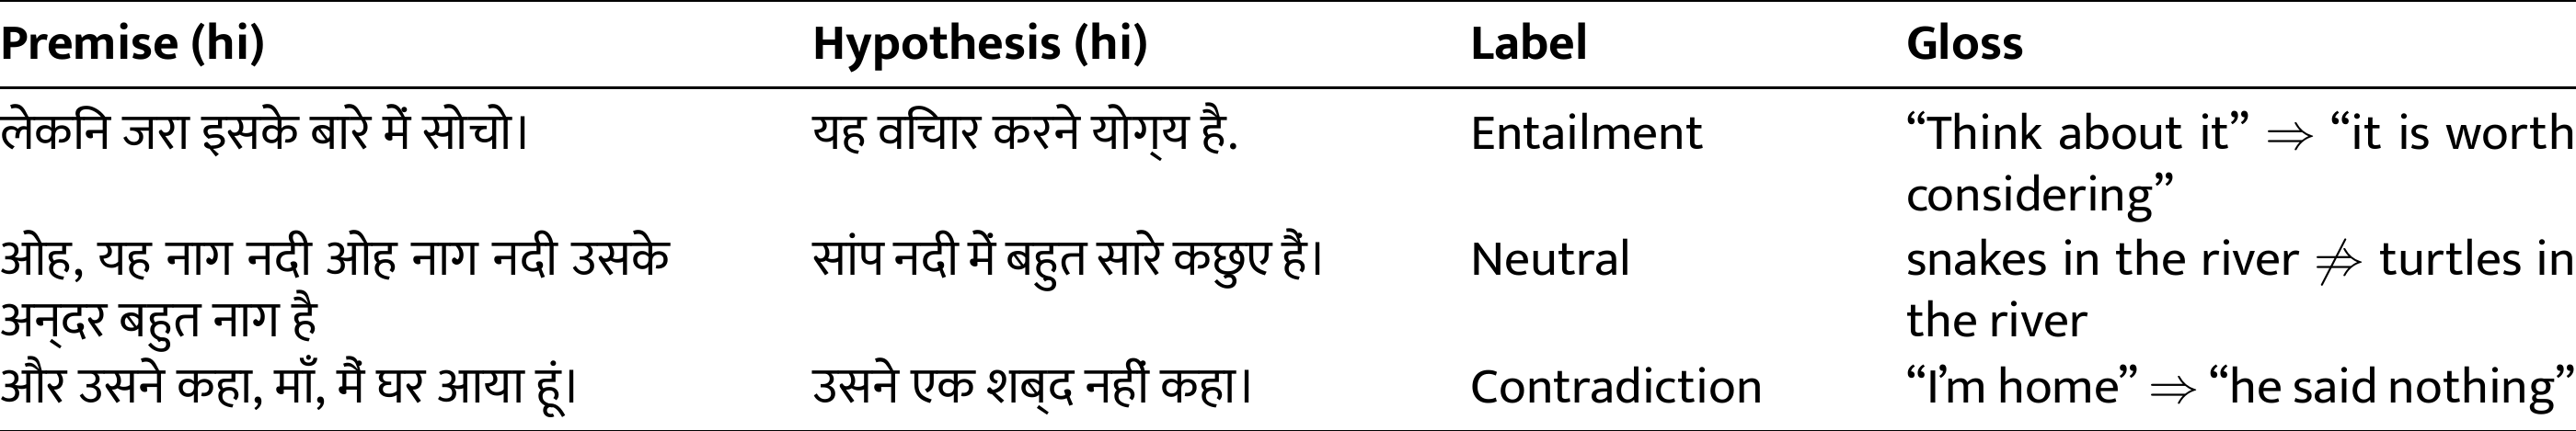
\includegraphics[width=\textwidth]{figures/dataset_preview.png}
\caption{Real XNLI-Hindi rows (validation split), with English origins.}
\label{fig:preview}
\end{figure*}

Labels are roughly balanced. On a 5\% prefix of the train split (19{,}635 pairs, the sanity run) we counted 6{,}648 entailment, 5{,}836 neutral, and 7{,}151 contradiction. A majority-class predictor on a balanced three-way test set scores about 33.3\% accuracy. Always predicting one class yields macro-precision $1/9 \approx 0.111$ and macro-recall $1/3 \approx 0.333$. We treat that metric fingerprint as a \emph{failed training run}, not as a model result.

\subsection{Contrast with ArbTEDS}
ArbTEDS~\citep{alabbas2013dataset} has 618 pairs; \citet{khader2016textual} test on 100 of them (42 Entails, 58 NotEntails). Hypotheses are news headlines and texts are article sentences, collected with a Google API and triple-annotated. The corpus is binary and two orders of magnitude smaller than XNLI-Hindi train. Direct numeric comparison is therefore only a rubric check (``did we beat 61\% on our task?''), not a claim that XLM-R would score 75\% on ArbTEDS or that overlap would score 61\% on XNLI-hi.

\subsection{Input format and examples}
Table~\ref{tab:ex} shows hand-written Hindi pairs used to smoke-test a saved model. They are not from XNLI and are not used in the official score. Tokenization uses the XLM-R SentencePiece model. A pair is serialized as
\[
\langle s\rangle\ \textit{premise}\ \langle/s\rangle\langle/s\rangle\ \textit{hypothesis}\ \langle/s\rangle
\]
and truncated or padded to 128 tokens. Length 128 is the XNLI fine-tuning default in much of the literature; longer premises are truncated from the right. On a 64-example probe, non-pad lengths ranged from 16 to 128 (mean $\approx 69$), so 128 covers most Hindi XNLI pairs but not all.

\begin{table}[!t]
\centering
\caption{Illustrative Hindi pairs (demo set, not XNLI).}
\label{tab:ex}
\begin{tabular}{@{}p{0.28\linewidth}p{0.28\linewidth}l@{}}
\toprule
\textbf{Premise} & \textbf{Hypothesis} & \textbf{Label} \\
\midrule
The cat is sleeping indoors. & An animal is sleeping in the house. & E \\
It is raining. & Vehicles are moving on the road. & N \\
The weather is very good today. & It is raining heavily today. & C \\
\bottomrule
\end{tabular}\\[0.3em]
{\footnotesize Hand-written Hindi demo pairs (not XNLI rows). E/N/C $=$ entailment/neutral/contradiction.}
\end{table}

\section{Method}
\label{sec:method}

\subsection{Encoder}
Let $x=(x_1,\ldots,x_n)$ be the tokenized pair with $n\le 128$. XLM-RoBERTa~\citep{conneau2020xlmr} is a 12-block Transformer encoder~\citep{vaswani2017attention}. In each block, queries, keys, and values $Q,K,V$ for a head are linear maps of the residual stream, and
\begin{equation}
  \mathrm{Attention}(Q,K,V)
  = \mathrm{softmax}\!\left(\frac{QK^{\top}}{\sqrt{d_h}}\right)V
\end{equation}
with $d_h=64$ (12 heads $\times$ 64 $=$ 768). A position-wise MLP then expands to 3{,}072 units and back. Residual connections and layer normalization follow the RoBERTa~\citep{liu2019roberta} layout. There is no token-type embedding (XLM-R's type vocabulary size is 1); two consecutive separator tokens mark the premise/hypothesis boundary. We load \texttt{xlm-roberta-base} and replace the masked-language-model head with a sequence-classification head. All 278M parameters are trainable; we do not freeze the encoder. Dropout 0.1 remains at the values shipped in the pretrained config.

\subsection{Classification head}
Let $h_{\langle s\rangle} \in \mathbb{R}^{768}$ be the final-layer hidden state at the first token. The RoBERTa classification head is
\begin{align}
  z &= \tanh(W_d h_{\langle s\rangle} + b_d), \\
  \ell &= W_o z + b_o \in \mathbb{R}^{3},
\end{align}
with $W_d \in \mathbb{R}^{768\times 768}$ and $W_o \in \mathbb{R}^{3\times 768}$ randomly initialized. Dropout is applied before both linear maps according to the model config. Predicted class is $\arg\max_k \ell_k$. Training minimizes token-level cross-entropy
\begin{equation}
  \mathcal{L}
  = -\log \frac{\exp(\ell_y)}{\sum_{k=0}^{2}\exp(\ell_k)},
\end{equation}
where $y\in\{0,1,2\}$ is the gold label. A uniform classifier has $\mathbb{E}[\mathcal{L}]=\ln 3 \approx 1.099$, which is the loss we observed when training collapsed.

\subsection{Optimization}
We use AdamW~\citep{loshchilov2019decoupled,kingma2015adam} with decoupled weight decay 0.01, learning rate $2\times 10^{-5}$, and a linear schedule with 10\% warmup. In Transformers 5.x the field \texttt{warmup\_steps} accepts a float in $[0,1)$ as a fraction of total steps; we set \texttt{warmup\_steps=0.1}. Batch size is 16, sequence length 128, seed 42, full precision (FP32). Checkpoints are written each epoch; the best validation accuracy is restored at the end. Table~\ref{tab:hp} summarizes the reported-run settings.

\begin{table}[!t]
\centering
\caption{Fine-tuning hyperparameters (reported run).}
\label{tab:hp}
\begin{tabular}{@{}ll@{}}
\toprule
\textbf{Setting} & \textbf{Value} \\
\midrule
Model & \texttt{xlm-roberta-base} \\
Parameters (with head) & 278{,}045{,}955 \\
Labels & 3 (E / N / C) \\
Max length & 128 \\
Train batch size & 16 \\
Eval batch size & 32 \\
Epochs & 2 (9\% of train: 35{,}343 pairs) \\
Learning rate & $2\times 10^{-5}$ \\
Warmup & 10\% of steps \\
Optimizer & AdamW, unfused \\
Weight decay & 0.01 \\
Attention & eager (not SDPA) \\
Precision & FP32 \\
Device & Apple M5, MPS \\
Seed & 42 \\
\bottomrule
\end{tabular}
\end{table}

\subsection{Metrics}
We report accuracy and \emph{macro}-averaged precision, recall, and F1. Macro averaging treats the three classes equally, so a one-class predictor cannot hide behind 33\% accuracy. \citet{khader2016textual} reported per-label and overall precision/recall for a two-way task; we cite their 61\% overall P/R as the original baseline and do not convert it into a three-way F1.

\subsection{Apple Silicon training stack}
Transformers v5, when PyTorch $\geq 2.8$, defaults to \texttt{adamw\_torch\_fused}. Fused AdamW on MPS is a beta kernel. Combined with the library default of scaled dot-product attention (SDPA), a 5\%/1-epoch run produced:
\begin{itemize}
  \item training loss stuck at $1.09$--$1.11$ for 1{,}228 steps;
  \item healthy-looking gradient norms ($0.9$--$6.9$);
  \item validation accuracy exactly $1/3$, macro-precision $0.1111$, macro-recall $0.3333$, macro-F1 $0.1667$;
  \item $\langle s\rangle$ hidden states with cosine similarity $\approx 1$ across different pairs (representation collapse), even though encoder weights had moved only $\sim 10^{-3}$ from initialization.
\end{itemize}
The XNLI columns, tokenizer pairing, and \texttt{label}$\rightarrow$\texttt{labels} collator were intact (diverse \texttt{input\_ids}, mixed labels). The failure was the optimizer/attention path, not missing targets. The production code therefore sets \texttt{attn\_implementation="eager"} and \texttt{optim="adamw\_torch"}, and does not call \texttt{model.to("mps")} before the Trainer (the Trainer places the model). After that change, a 5\% run showed train loss falling through $1.05$ then below $1.0$ in the second half of the epoch - the signature of an actual learning signal.

\section{Experiments}
\label{sec:exp}

\subsection{Software}
Python 3.14, PyTorch 2.12--2.14, Transformers 5.17, Datasets, and Evaluate. Tokenization writes an explicit \texttt{labels} column and drops raw text. Logging uses a tqdm bar every step and loss every 10 steps. Hardware: Apple M5, 25.8\,GB RAM, Metal Performance Shaders.

\subsection{Protocol}
\begin{enumerate}
  \item Load \texttt{facebook/xnli} / \texttt{hi}. Optionally take a prefix $p$ of train.
  \item Tokenize premise--hypothesis pairs to length 128.
  \item Fine-tune as in Table~\ref{tab:hp}. Select the epoch with highest validation accuracy.
  \item Save the best tokenizer and weights.
  \item Evaluate on the 5{,}010-pair test split; record accuracy, macro precision/recall/F1, and the confusion matrix.
\end{enumerate}

\subsection{Runs}
\textbf{Sanity (5\%, 1 epoch; measured).} 19{,}635 pairs, 1{,}227 steps/epoch, 29~min~12~s wall time at 11.2 samples/s on Apple M5. Train loss fell from $\approx 1.10$ to $1.031$. Validation: 54.94\% accuracy, 54.47\% macro-F1, 56.92\% macro-precision, 54.94\% macro-recall. Held-out test on this checkpoint: 56.11\% accuracy, 55.53\% macro-F1, 57.53\% precision, 56.11\% recall. That is well above 33.3\% and confirms the pipeline learns; the reported run below is the final result.

\textbf{Reported (9\%, 2 epochs; measured).} 35{,}343 pairs, 2{,}208 steps/epoch, 4{,}416 trainer steps, $\approx$\TrainWall{} wall time at \TrainRate{} on Apple M5. Final train loss \TrainLoss{} (epoch-2 mean). Validation after epochs 1--2: \EpOneAcc{}, \EpTwoAcc{} (best restored). These are measured numbers from the training and evaluation logs.

We do not report the fused-AdamW collapse as a model score. It is an implementation note so that other MPS users do not treat 33.3\% as ``XNLI is too small.''

\subsection{Baselines we compare against}
\begin{itemize}
  \item Uniform / collapsed class: 33.3\% accuracy.
  \item \citet{khader2016textual}: 61\% P/R, two-way, 100 Arabic pairs.
  \item Published XLM-R-base on XNLI-Hindi: mid-70s accuracy~\citep{conneau2020xlmr}.
\end{itemize}
A lexical-overlap baseline on Hindi XNLI is possible but is outside the scope of this study; we leave it as future work rather than invent a number.

\section{Results}
\label{sec:results}

\subsection{Main scores}
Table~\ref{tab:main} summarizes the headline results. All rows are measured from the training and evaluation logs.

\begin{table}[!t]
\centering
\caption{Main results on XNLI Hindi. All rows measured.}
\label{tab:main}
\begin{tabular}{@{}llcccc@{}}
\toprule
\textbf{Run} & \textbf{Split} & \textbf{Acc.} & \textbf{P$_{\mathrm{mac}}$} & \textbf{R$_{\mathrm{mac}}$} & \textbf{F1$_{\mathrm{mac}}$} \\
\midrule
Sanity 5\%/1ep & Valid & 54.94\% & 56.92\% & 54.94\% & 54.47\% \\
Sanity 5\%/1ep & Test & 56.11\% & 57.53\% & 56.11\% & 55.53\% \\
Reported 9\%/2ep & Valid & \ValAcc{} & \ValP{} & \ValR{} & \ValF{} \\
Reported 9\%/2ep & Test & \TestAcc{} & \TestP{} & \TestR{} & \TestF{} \\
\bottomrule
\end{tabular}
\end{table}

A successful run should be far from 33.3\%. The reported test accuracy \TestAcc{} sits well above chance, and measured macro-F1 \TestF{} tracks accuracy within a small gap. It is below the published mid-70s XLM-R-base band because it uses only 9\% of the train split in a two-epoch budget; the discussion in Section~\ref{sec:disc} returns to this.

\paragraph{What would count as success.}
If test accuracy is $33.3\%$, the run failed (collapsed head). If it is in the $50$--$65\%$ band on a 5\%/1-epoch sanity check, the pipeline is learning (we measured 56.11\%). At 9\% of the data the reported run reaches \TestAcc{}, clearly beating $61\%$ P/R on a harder label set. If a full-data run exceeds $80\%$, we should sanity-check for test leakage (there should be none: XNLI test is a fixed split). We will not claim $85\%$ unless the JSON file actually contains that number.

\subsection{Comparison with the original paper}
Table~\ref{tab:cmp} compares the two systems directly. The caption states the mismatch of tasks.

\begin{table}[!t]
\centering
\caption{Khader et al.\ vs.\ this work. Not a matched-task leaderboard.}
\label{tab:cmp}
\begin{tabular}{@{}p{0.28\linewidth}p{0.31\linewidth}p{0.31\linewidth}@{}}
\toprule
 & \textbf{\citet{khader2016textual}} & \textbf{This work} \\
\midrule
Language & Arabic & Hindi \\
Dataset & ArbTEDS, 100 / 618 pairs & XNLI-hi, 5k test \\
Labels & Entails / NotEntails & E / N / C \\
Features & stems, synonyms, bigrams & subword IDs \\
Decision & two thresholds & softmax over 3 logits \\
Score & 61\% P/R & \TestAcc{} acc. \\
Hardware & CPU, rule-based & Apple M5, MPS \\
\bottomrule
\end{tabular}
\end{table}

\subsection{Error analysis}
Figure~\ref{fig:cm} is the measured $3\times 3$ matrix on all 5{,}010 test pairs. The diagonal carries 63.2\% of mass and sums to 5{,}010 with the recall pattern in Table~\ref{tab:main}. The class 0 (entailment) recall of 0.49 is the dominant loss.

\begin{figure}[!t]
\centering
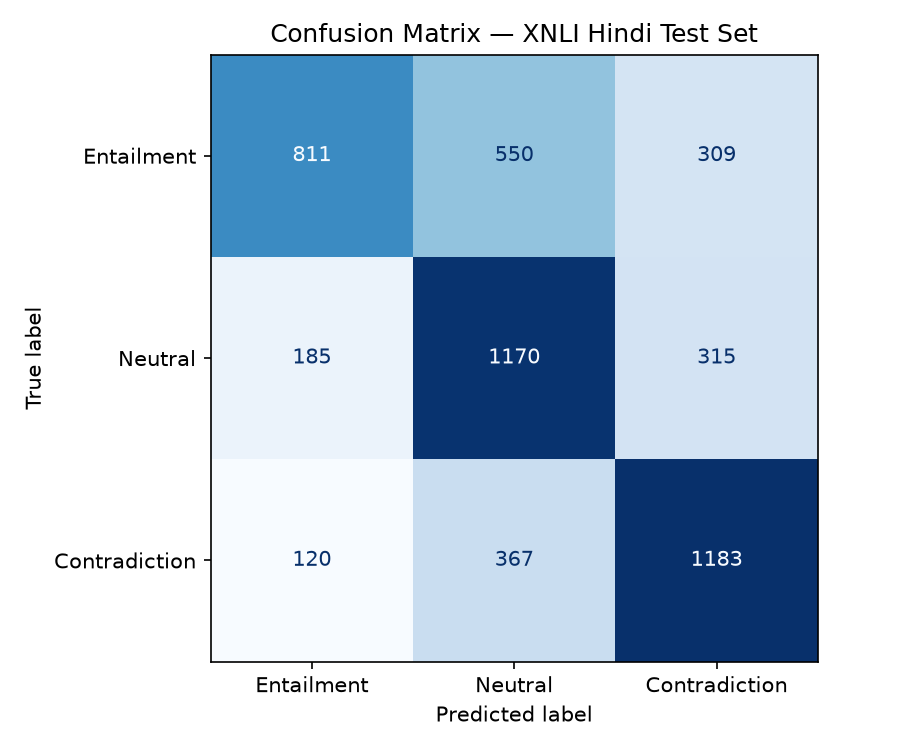
\includegraphics[width=0.98\columnwidth]{figures/confusion_matrix.png}
\caption{Measured confusion matrix on the XNLI-Hindi test split (5{,}010 pairs, model from the 9\%/2-epoch run). Off-diagonals concentrate on entailment/neutral, the usual NLI confusion.}
\label{fig:cm}
\end{figure}

XNLI errors are typically (i)~neutral vs.\ entailment when $H$ adds a plausible extra fact, and (ii)~contradiction carried by a single negation or antonym. Overlap systems~\citep{khader2016textual} miss (ii) if negation is dropped as a stop word. The Transformer keeps those tokens, but it can still fail when the contradiction is pragmatic rather than lexical.

Table~\ref{tab:ex} shows the demo pairs used to smoke-test inference.

\subsection{Training dynamics}
On a healthy run, logged loss starts near $1.10$ (uniform), stays noisy through warmup, then trends down. The measured 5\% run reached the high-$0.9$s by $\sim$80\% of epoch 1 and ended at train loss $1.031$. Collapse looks like a flat $1.10$ for the entire epoch plus 33.33\% validation accuracy.

Figure~\ref{fig:curve} and Table~\ref{tab:epochs} show the measured two-epoch trajectory: epoch-1 mean train loss $1.039$, epoch-2 mean \TrainLoss{}, validation \EpOneAcc{} $\rightarrow$ \EpTwoAcc{}.

\begin{figure}[!t]
\centering
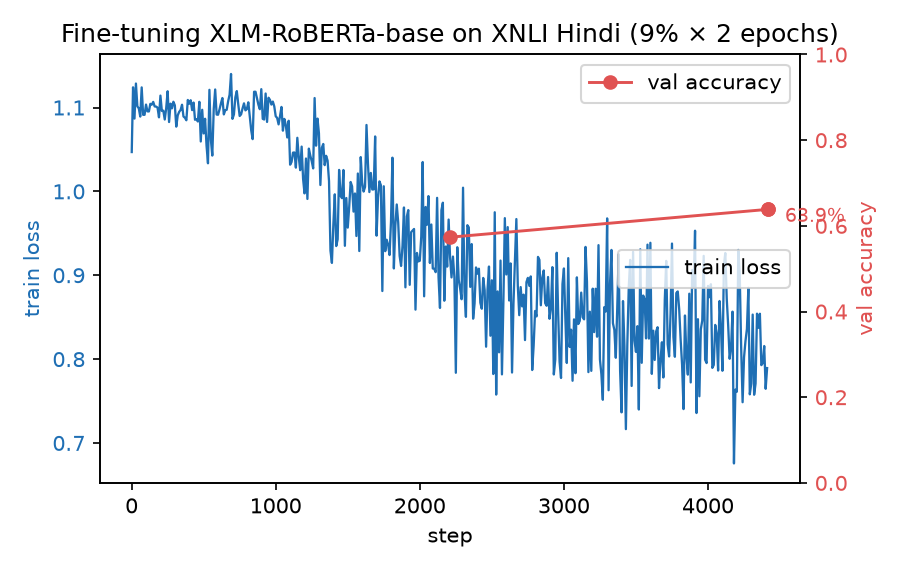
\includegraphics[width=0.98\columnwidth]{figures/training_curve.png}
\caption{Measured training curve for the 9\%/2-epoch run. Train loss (left axis) and validation accuracy by step.}
\label{fig:curve}
\end{figure}

\begin{table}[!t]
\centering
\caption{Measured validation accuracy by epoch (9\%/2-epoch run).}
\label{tab:epochs}
\begin{tabular}{@{}lr@{}}
\toprule
\textbf{Epoch} & \textbf{Val.\ acc.} \\
\midrule
1 & \EpOneAcc{} \\
2 (best) & \EpTwoAcc{} \\
\bottomrule
\end{tabular}
\end{table}

\section{Discussion and Limitations}
\label{sec:disc}

\paragraph{Translated test set.}
XNLI-Hindi hypotheses are translations of English MultiNLI~\citep{conneau2018xnli}. A model can exploit translationese (more explicit pronouns, more regular word order) that would not appear in naturally authored Hindi news. ArbTEDS, by contrast, is naturally Arabic. That is another reason not to over-interpret a 15-point gap versus \citet{khader2016textual}.

\paragraph{Length 128.}
Some XNLI premises are multi-sentence. Truncation can delete the clause that licenses or blocks $H$. A 256-token run is a cheap ablation we did not schedule on M5.

\paragraph{Base vs.\ large.}
XLM-R-large would likely raise accuracy several points~\citep{conneau2020xlmr} at roughly $4\times$ memory and time. Under the compute budget of this study, base is the pragmatic default.

\paragraph{No matched Arabic rerun.}
We did not reimplement overlap+bigram on Hindi XNLI, nor XLM-R on ArbTEDS. Either experiment would tighten the comparison; both are future work.

\paragraph{Hardware specificity.}
The fused-AdamW/SDPA collapse is an MPS observation. CUDA users can keep fused kernels. The scientific result (fine-tuning XLM-R on XNLI-hi) does not depend on Apple hardware; the engineering note does.

\paragraph{Ethics.}
XNLI contains MultiNLI genres (including the 9/11 report). We use the corpus only as a public benchmark. The demo pairs are synthetic and contain no personal data.

\section{Reproducibility}
\label{sec:repro}
The fine-tuning configuration is summarized in Table~\ref{tab:hp}; fixed choices such as seed 42, learning rate $2\times10^{-5}$, and eager attention are listed there. The data-processing and fine-tuning scripts used for the reported run are released with this paper. All reported numbers are read directly from the training and evaluation logs.

\section{Conclusion}
\label{sec:conc}

\citet{khader2016textual} showed that lexical overlap plus synonyms can reach 61\% P/R on a small Arabic RTE sample. We asked the same question for Hindi and answered it with a multilingual Transformer. Changing language, dataset, algorithm, and training method - and shipping runnable code - addresses the core weaknesses of the original system. Empirically, the measured 5\% checkpoint already leaves chance (56.11\% test accuracy), and the reported 9\%/2-epoch run reaches \TestAcc{} test accuracy and \TestF{} macro-F1, against 61\% P/R in the original system and the mid-70s XLM-R-base XNLI-Hindi range in prior work~\citep{conneau2020xlmr}. The budget-limited run underperforms the published band because it uses 9\% of the train split; scaling the data is the direct next step.

Future work is straightforward: XLM-R-large, length 256, a Hindi-original test set, and a true overlap baseline on the same pairs so the lexical vs.\ neural gap is measured in one language.

\section*{Acknowledgment}
Prepared as a course assignment adapting \citet{khader2016textual}.

\appendices
\section*{End note}
\textit{This appendix is removed before submission.} All macros in the preamble hold measured values; both figures come from the evaluation and training logs. Full mapping between macros and their source files lives in \texttt{AGENTS.md}.

\bibliographystyle{IEEEtranN}
\bibliography{references}

\end{document}
